\scanpage{75}
\[
\sum_1^n\log(1+r\rho_i(u+v))\leq\sum_1\log(1+r\rho_i(u))+\sum_1\log(1+r\rho_i(v))
\]

\[
S_{\deleted{\unsure{m}}\varphi}^{n}(u+v)\leq S_\varphi^n(u)+S_\varphi^n(v)\qquad S_\varphi^n(w)=\sum_1^n f_\varphi(\rho_i(w))
\]

\[
f_\varphi(\rho)=\int_0^{+\infty}\frac{\varphi(r)}{\frac1\rho+r}\,dr=\int_0^{+\infty}\varphi\left(\frac s\rho\right)\frac{ds}{1+s}
\]

$\varphi$ decreasing function

(motivation : \inserted{If $A(0)=B(0)=0$ ($=0$ is a \unsure{symbol|example}), then} $A(r)\leq B(r)$ for $0\leq r\leq+\infty$ is equivalent to $\int\psi(r)A(r)\,dr\leq\int\psi(r)B(r)\,dr$ for every $\psi\geq0$ with compac\textsuperscript{t} support in $[a,b]$, Now, setting $\psi(r)=-\varphi'(r)$, $\varphi$ \inserted{\uline{continuously} \uline{differentiable}} \unsure{decreasing} function, zero at $b$ : \deleted{(\unsure{continuously}} \unsure{\deleted{\inserted{zero}}|\inserted{zero}} \deleted{\unsure{continuous at} \illegible{1}} (which is $+\infty$) and supposing \deleted{\unsure{of}}

that $A$ is differentiable $-\int\varphi'(r)A(r)\,dr=[-\varphi(r)A(r)]_0^{+\infty}+\int\varphi(r)A'(r)\,dr$ and the first term is zero, whence $\int\varphi(r)A'(r)\,dr$. If therefore $A$ and $B$ are differentiable, then we therefore obtain

\[
\int\varphi(r)A'(r)\,dr\leq\int\varphi(r)B'(r)\,dr
\]

for every continuously differentiable function $\varphi$, decreasing \inserted{on $[0,+\infty[$} and zero in a neighborhood of $+\infty$. If in addition $A'(r)$, $B'(r)\geq0$, then this will be true for \deleted{every} \unsure{such} decreasing function or zero, possibly infinite. (If we take

$\varphi=$

\figure{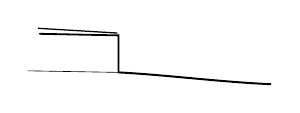
\begin{tikzpicture}[x=1mm,y=1mm,line cap=round]\draw[line width=.16mm] (0,5.6)--(10,5.0);\draw[line width=.23mm] (.2,4.9)--(10.2,4.7)--(10.2,0);\draw[line width=.08mm] (-1.3,.2)--(10.2,0);\draw[line width=.25mm] (10.2,0)..controls(16,-.3)and(23,-1.2)..(29.5,-1.5);\end{tikzpicture}}

, we recover $A(r)\leq B(r)$). In the present case,

\[
A\deleted{\unsure{^{\,\prime}|{}^{\sim}}}(r)=\sum_1^n\log(1+r\rho_i(u))\qquad \text{thus }\ A'(r)=\sum\frac{r}{1+r\rho_i(u)}
\]

whence our assertion. -- The most important case is the one where we take $\varphi(r)=r^{-p}$ $0<p<1$. We then find

\margin{76}
